\apendice{Especificación de diseño}

\section{Introducción}
En este apartado se va a tratar la especificación de diseño desarrollado a lo largo de este proyecto, dividido en diferentes apartados considerados clave para el éxito del desarrollo de esta web. Una buena especificación de diseño nos ha permitido, partiendo de la idea inicial de cliente, transformar sus necesidades en un producto final completo apoyándonos en un sistema lo más estructurado y eficaz posible.

\section{Diseño del modelo datos}
La aplicación web contiene una serie de entidades que aseguran el cumplimiento de los requerimientos:
\begin{itemize}
    \item \textbf{Libros:} Esta entidad almacena información sobre los libros disponibles en el sistema. Incluye detalles como el título, ISBN, editorial, descripción, año de publicación, puntuaciones y ubicaciones del estudio.
    \item \textbf{LibrosAutomaticos:} Almacena información de manera temporal acerca los libros obtenidos mediante web scraping, incluyendo detalles como título, ISBN, editorial y descripción.
    \item \textbf{Fecha\_modificacion:} Registra la última fecha y hora de modificación de los datos del catálogo, indicando así a los usuarios si han existido modificaciones y cuando.
    \item \textbf{GestionEstimacion:} Contiene detalles de las actividades de producción, poder y mantenimiento tanto de hombres como de mujeres, necesarias para realizar valoraciones de libros.
    \item \textbf{Roles:} Define los diferentes roles disponibles en el sistema, como administrador, usuario, etc. Cada rol puede estar asociado con múltiples usuarios.
    \item \textbf{Usuarios:} Almacena información sobre los usuarios del sistema, incluyendo su nombre, correo electrónico, contraseña encriptada y el rol asignado.
    \item \textbf{Botones:} Contiene información sobre los diferentes botones de la interfaz del sistema y los roles autorizados para utilizarlos, permitiendo un ajuste dinámico de permisos en base a roles.
    \item \textbf{Estimacion:} Registra las estimaciones realizadas por los usuarios, incluyendo detalles sobre género, actividades, ubicación, título e ISBN del estudio, y los resultados obtenidos.
    \item \textbf{EstadisticasPorMes:} Almacena estadísticas mensuales de los libros, como el número de libros, visitas totales, estimaciones, usuarios y el libro más visitado.
    \item \textbf{EstadisticasPorMesAuxiliar:} Similar a EstadisticasPorMes, pero utilizada como una entidad auxiliar durante la importación de catálogo y almacenamiento temporal.
    \item \textbf{Colaboradores:} Almacena información sobre los colaboradores de valoraciones de libros, incluyendo su nombre, apellido e institución.
\end{itemize}

Tras mencionar todas las entidades existentes, cabe destacar que todas las entidades son independientes unas de otras excepto dos, la entidad Usuarios y la entidad Roles, ya que todo usuario debe de tener asignado un solo rol, pero un rol puede estar asignado para varios roles. Esto se ve de manera más visual en el diagrama relacional de la figura \ref{Diagrama Relacional}:

\begin{figure}[htbp]
    \centering
    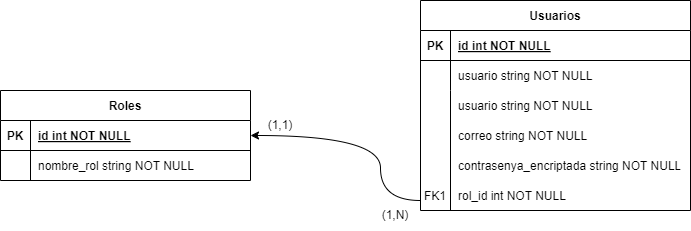
\includegraphics[width=0.9\linewidth]{Imagenes/Diagrama relacional.png}
    \caption{Diagrama Relacional}
    \label{Diagrama Relacional}
\end{figure}
\FloatBarrier

\section{Diseño procedimental}
En este apartado se van a mostrar mediante diagramas de flujo algunos de los procedimientos internos más interesantes y de mayor complejidad de este proyecto.

En el diagrama de flujo de la figura \ref{Diagrama de flujo Web scraping Frontend} podemos apreciar todos los pasos que se realizan cuando un usuario quiere obtener un libro a través del web scraping desde el \textit{frontend}. En la figura \ref{Diagrama de flujo permisos Backend} se aprecia la parte del \textit{backend}, donde se ejecuta toda la lógica

\newpage
\subsubsection{\textit{Frontend}:}
\begin{figure}[htbp]
    \centering
    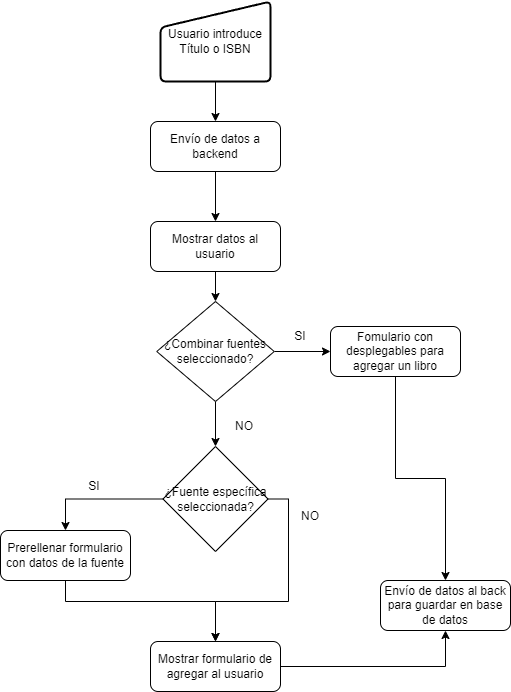
\includegraphics[width=0.7\linewidth]{Imagenes/Front web scraping.png}
    \caption{Diagrama de flujo Web scraping \textit{Frontend}}
    \label{Diagrama de flujo Web scraping Frontend}
\end{figure}
\FloatBarrier

\newpage
\subsubsection{\textit{Backend}:}
\begin{figure}[htbp]
    \centering
    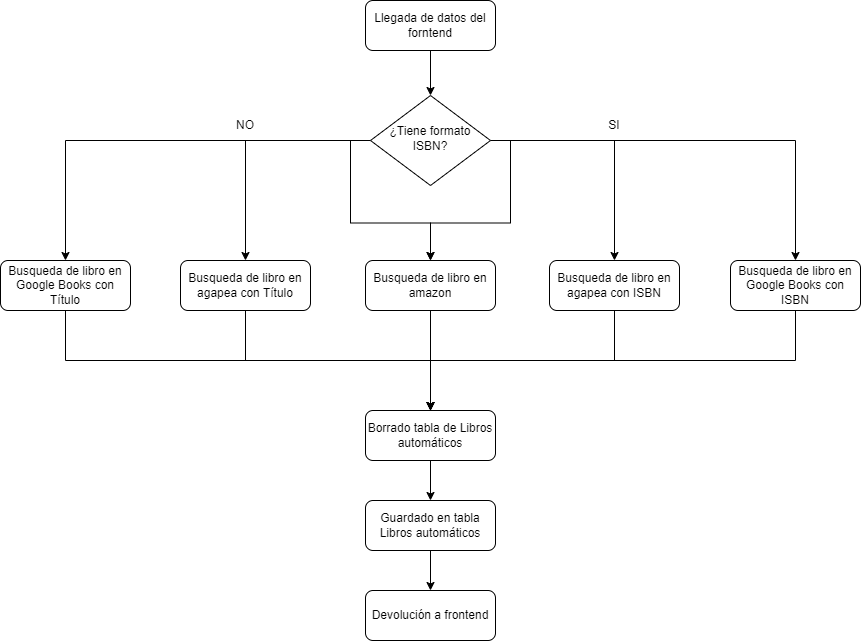
\includegraphics[width=1\linewidth]{Imagenes/Back web scraping.png}
    \caption{Diagrama de flujo Web scraping \textit{Backend}}
    \label{Diagrama de flujo Web scraping Backend}
\end{figure}
\FloatBarrier

En las figuras \ref{Diagrama de flujo permisos Frontend} y \ref{Diagrama de flujo permisos Backend} muestra el sistema que permite a la web bloquear o permitir la entrada dinámicamente a los usuarios a ciertas partes de la web utilizando permisos, los cuales no son estáticos y son editables.

\newpage
\subsubsection{\textit{Frontend}:}
\begin{figure}[htbp]
    \centering
    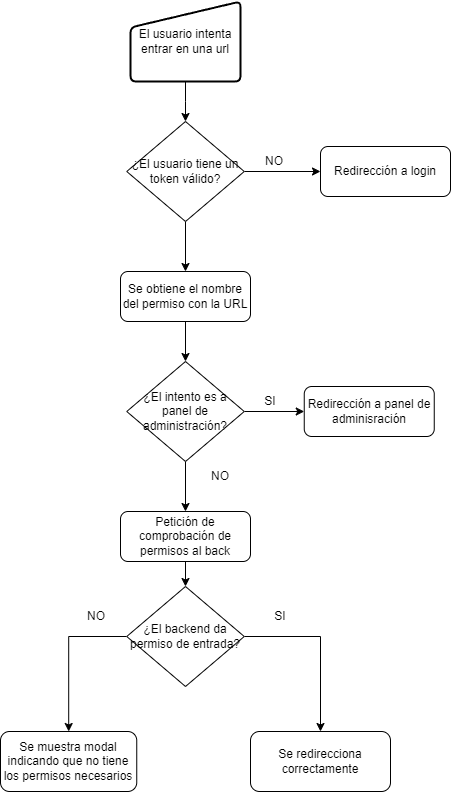
\includegraphics[width=0.6\linewidth]{Imagenes/Front permisos.png}
    \caption{Diagrama de flujo permisos \textit{Frontend}}
    \label{Diagrama de flujo permisos Frontend}
\end{figure}
\FloatBarrier

\newpage
\subsubsection{\textit{Backend}:}
\begin{figure}[htbp]
    \centering
    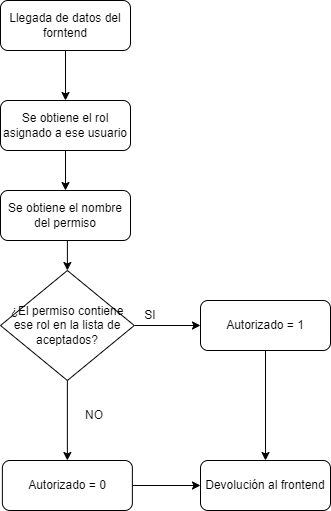
\includegraphics[width=0.5\linewidth]{Imagenes/Back permisos.png}
    \caption{Diagrama de flujo permisos \textit{Backend}}
    \label{Diagrama de flujo permisos Backend}
\end{figure}
\FloatBarrier

\section{Diseño de interfaces}
 Para realizar un primer prototipado del diseño de interfaz de la web se utilizó la herramienta Justimind, que ha permitido el diseño y la estructura de las funciones básicas de este proyecto.

A continuación, se muestran algunas de las interfaces realizadas con la herramienta:
\begin{figure}[htbp]
    \centering
    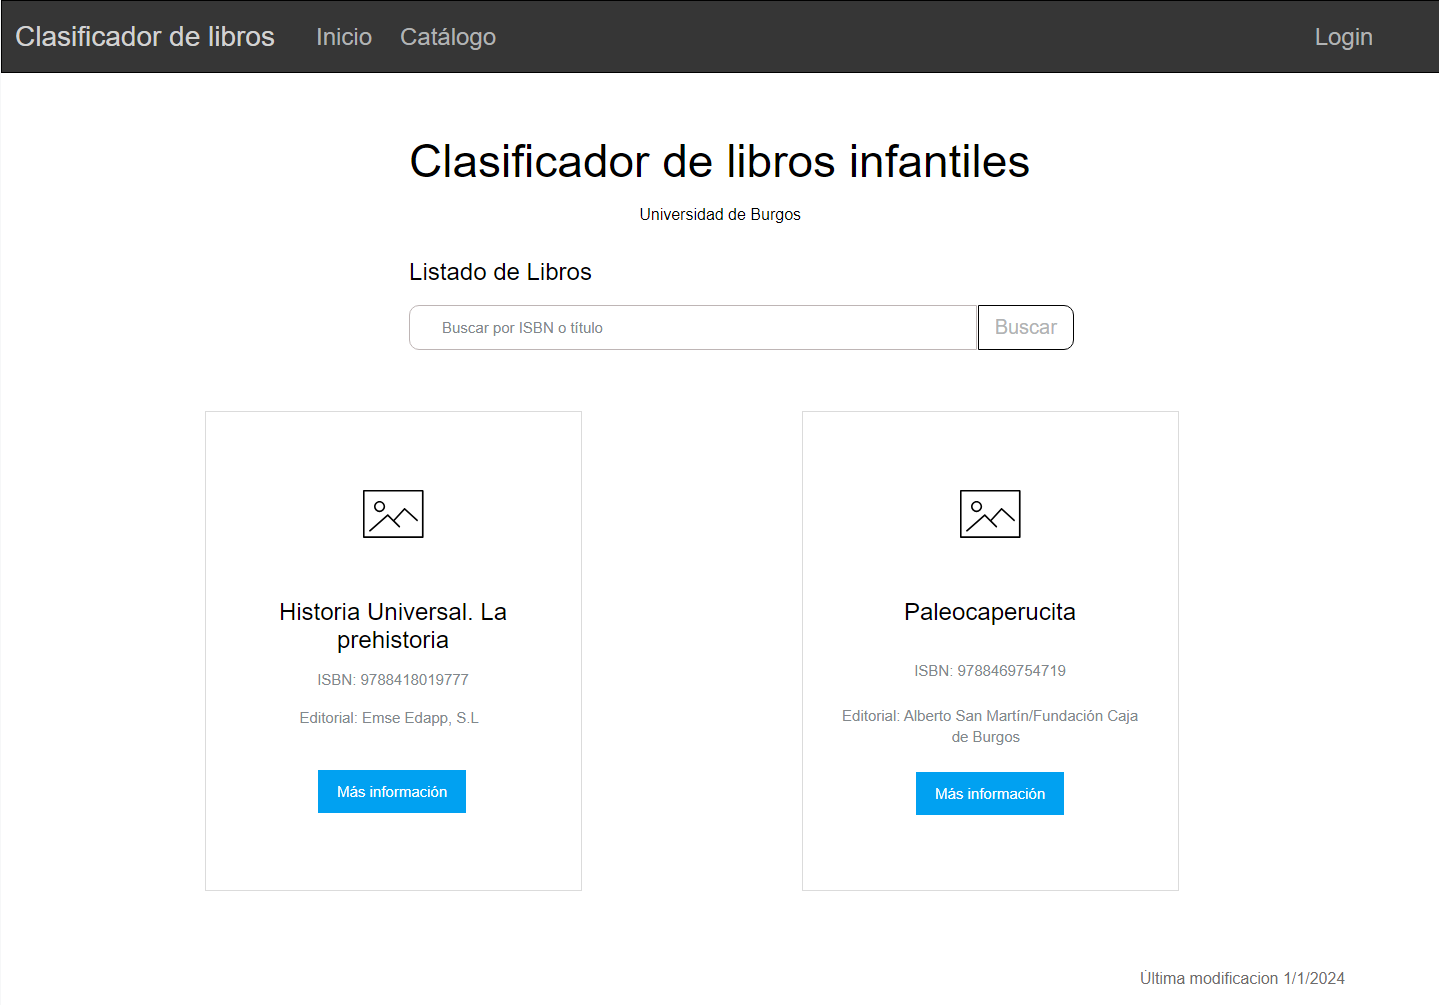
\includegraphics[width=0.9\linewidth]{Imagenes/PrototipoCatalogo.png}
    \caption{Prototipo catálogo}
    \label{Prototipo catálogo}
\end{figure}
\begin{figure}
    \centering
    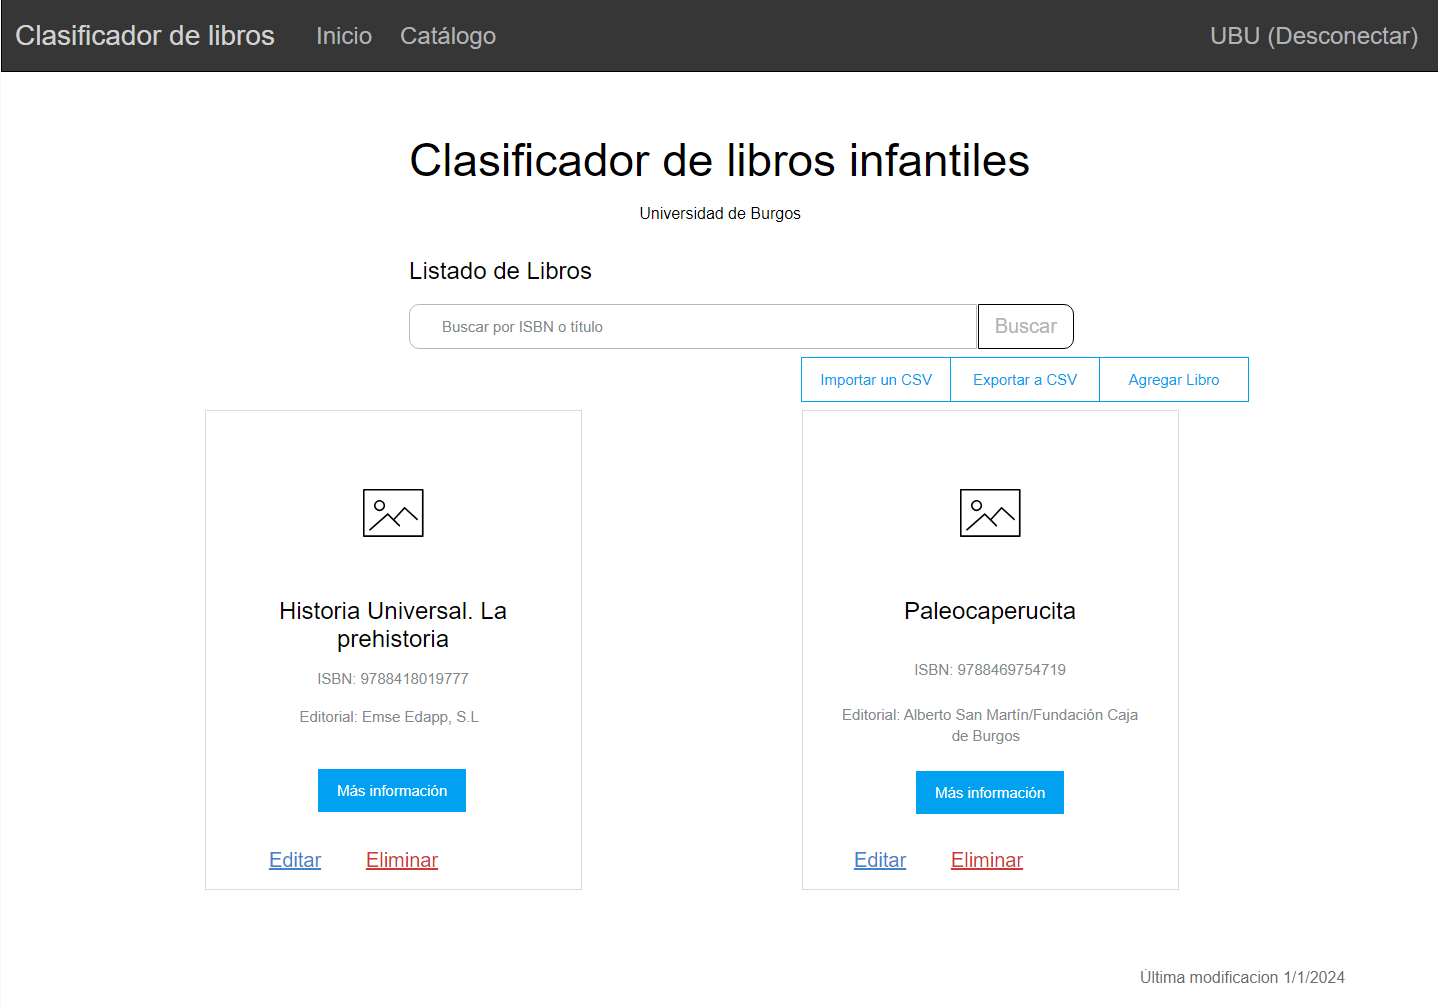
\includegraphics[width=0.9\linewidth]{Imagenes/CatalogoAdministrador.png}
    \caption{Prototipo catálogo (Vista de administrador)}
    \label{Prototipo catálogo (Vista de administrador)}
\end{figure}
\FloatBarrier

\begin{figure}[htbp]
    \centering
    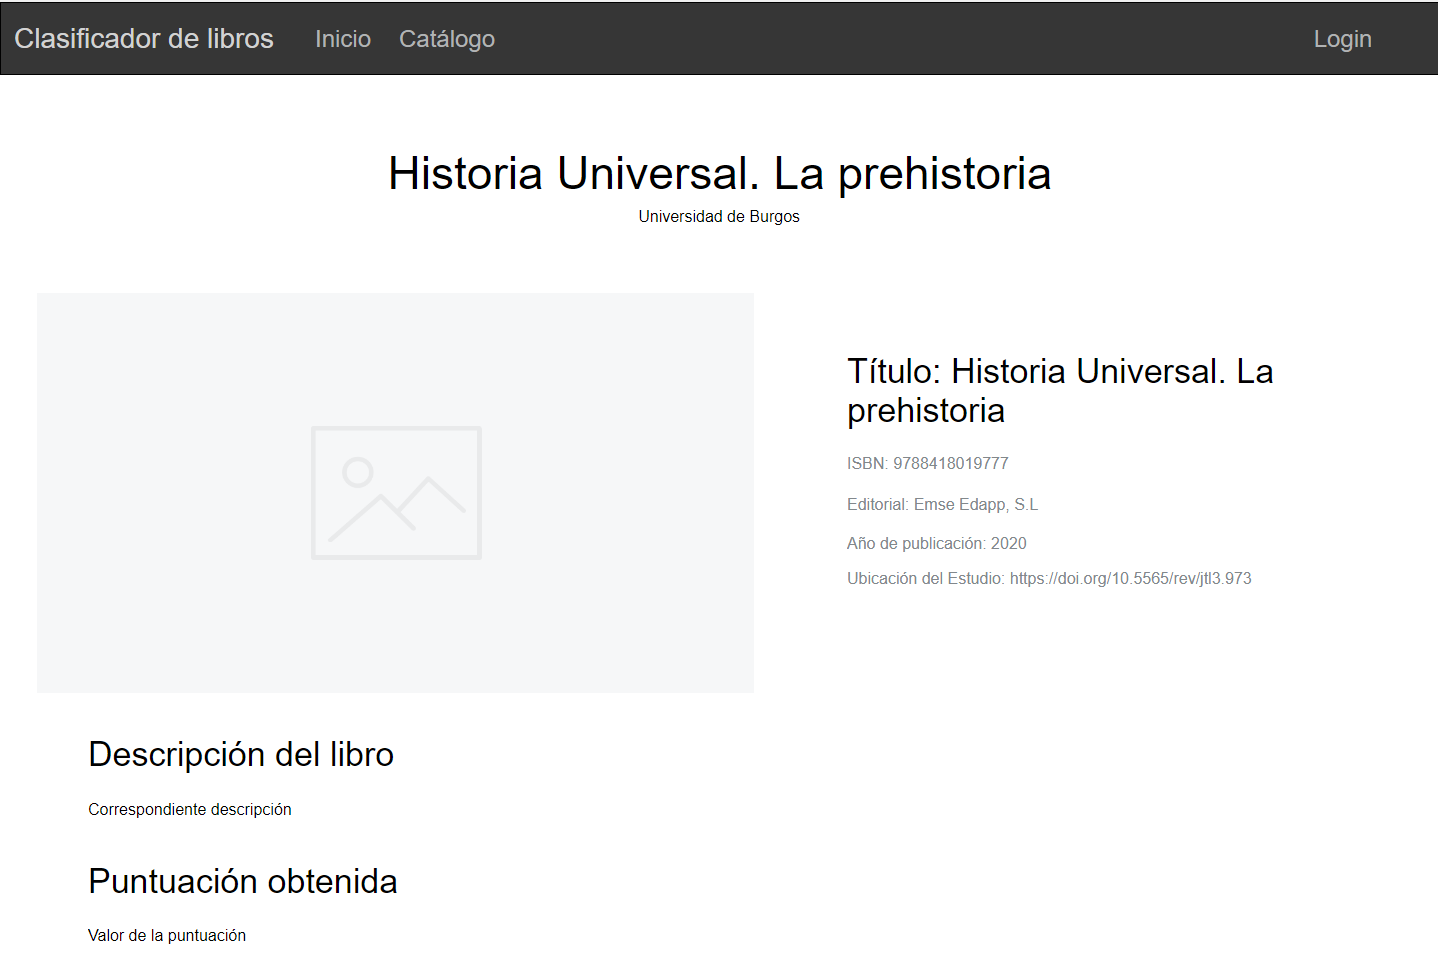
\includegraphics[width=0.9\linewidth]{Imagenes/PrototipoMasInfo.png}
    \caption{Prototipo Más Información}
    \label{Prototipo Más Información}
\end{figure}
\begin{figure}
    \centering
    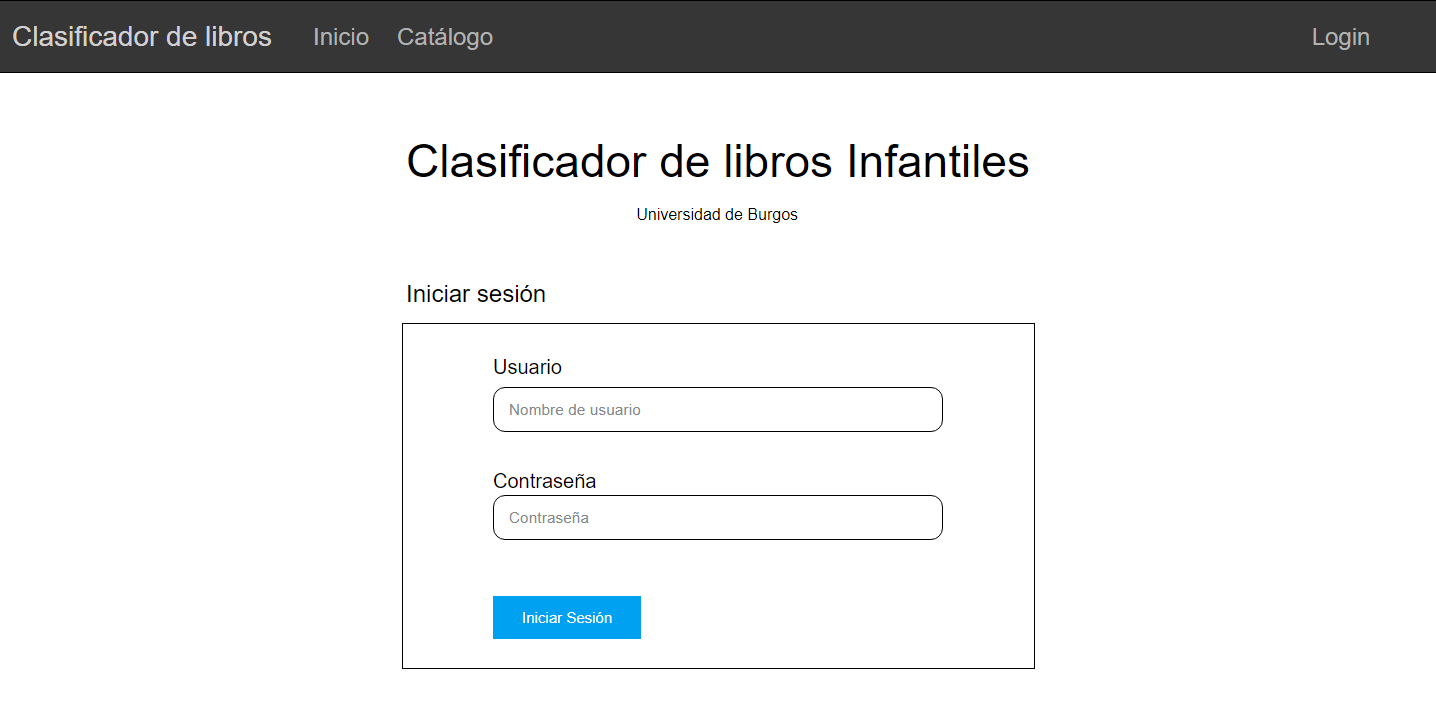
\includegraphics[width=0.9\linewidth]{Imagenes/PrototipoLogin.png}
    \caption{Prototipo Login}
    \label{Prototipo Login}
\end{figure}
\FloatBarrier

\section{Diseño de la arquitectura}
Dentro de este apartado se exponen los patrones de diseño utilizados durante el desarrollo de esta aplicación web. Para una mejor comprensión se separan los patrones de \textit{frontend} y \textit{backend} y finalmente la combinación de ambos.
\subsection{ Patrones del \textit{backend}}
\subsubsection{Patrón modular~\cite{PatrónMódulo}}
El patrón modular tiene como objetivo principal separar las funcionalidades del código en módulos separados y lo más independientes posibles. Cada módulo consiste en una o varias funcionalidades relacionadas entre sí. Esto contiene la gran ventaja de poder reutilizar el código y tener una escalabilidad y mantenibilidad muy simple y eficaz.

A nivel de ejemplo del \textit{backend}, en la figura \ref{Módulos backend} se puede apreciar cómo las funcionalidades principales se encuentran separadas en carpetas con sus correspondientes archivos, utilizando uno general para conectarlos entre si y poder usar todos los componentes.

\begin{figure}
    \centering
    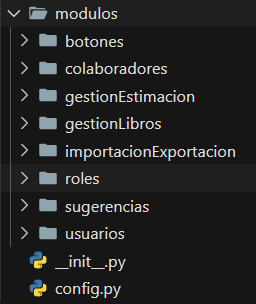
\includegraphics[width=0.5\linewidth]{Imagenes/Modulos.png}
    \caption{Módulos \textit{backend}}
    \label{Módulos backend}
\end{figure}


Un ejemplo más concreto de estos módulos es la carpeta gestionLibros, la cual es la encargada de toda la lógica relacionada con todas las operaciones del catálogo.

\begin{figure}[htbp]
    \centering
    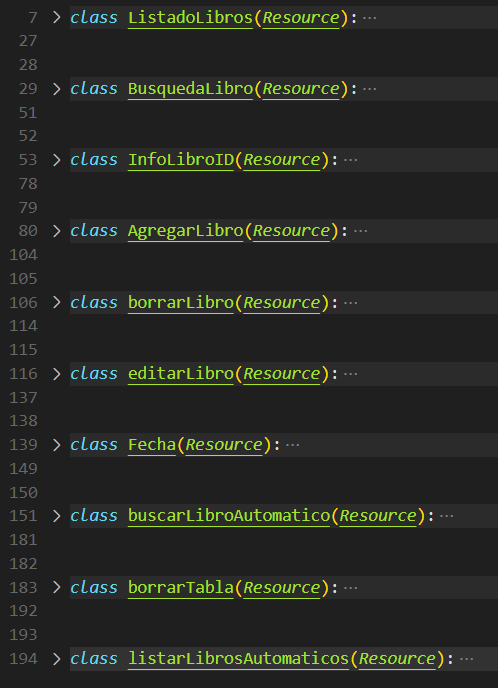
\includegraphics[width=0.5\linewidth]{Imagenes/Ejemplo gestionLibros.png}
    \caption{Funciones gestionLibros}
    \label{Funciones gestionLibros}
\end{figure}
\FloatBarrier

\subsubsection{Patrón repositorio\cite{PatrónRepositorio}}
El patrón repositorio es utilizado para permitir la separación entre el acceso a los datos de la base de datos con la lógica de negocio. Al realizar esta acción podemos tener grandes ventajas como son la limpieza, la mantenibilidad y la posibilidad de realización de pruebas unitarias de manera sencilla.

A nivel de ejemplo esto se puede apreciar en la estructura del proyecto al existir una separación entre todas los módulos de funcionalidades y el apartado de modelos.

\begin{figure}[htbp]
    \centering
    \includegraphics[width=0.4\linewidth]{Imagenes/Patrón repositorio.png}
    \caption{Patrón repositorio}
    \label{Patrón repositorio}
\end{figure}
\FloatBarrier

\subsection{Patrones del \textit{frontend}}
\subsubsection{Patrón de componentes~\cite{PatrónComponentes}}
El patrón de componentes consiste en dividir la interfaz del usuario en elementos totalmente independientes y reutilizables. Cada componente existente en el proyecto contiene su propia lógica y su propia y diseño, lo cual permite tener una modularización completa y muy fácilmente escalable. Este patrón es esencial para poder construir vistas muy complejas utilizando componentes muy pequeños.

Para ejemplificarlo, en la figura \ref{ComponentesAngular} se puede observar algunos de los componentes creados para la aplicación web, donde se observa la separación completa y los elementos de cada componente.
\begin{figure}
    \centering
    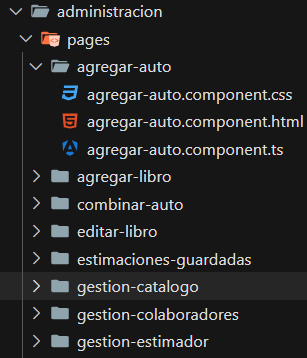
\includegraphics[width=0.4\linewidth]{Imagenes/ComponentesAngular.png}
    \caption{ComponentesAngular}
    \label{ComponentesAngular}
\end{figure}
\FloatBarrier

\subsubsection{Patrón de servicios~\cite{PatrónServicios}}
El patrón de servicios consiste en generar archivos que contengan la lógica que sea compartida por varios de los componentes. En el caso de este proyecto, los servicios se han utilizado para realizar las llamadas necesarias al \textit{backend}, definiendo así una serie de funciones que pueden compartir varios de los componentes existentes, en base a sus necesidades.
Para poder utilizar correctamente estos elementos, han de inyectarse en los constructores de todos aquellos componentes que quieran interactuar con ellos.

A modo de ejemplo, en la figura \ref{Servicio de libros} se puede ver una parte de uno de los servicios existentes (en este caso es el servicio de los libros), donde entre todos los elementos que contiene, se pueden observar las funciones que realizan las llamadas al \textit{backend} y una función donde se establecen las cabeceras de todas las llamadas.

\begin{figure}[htbp]
    \centering
    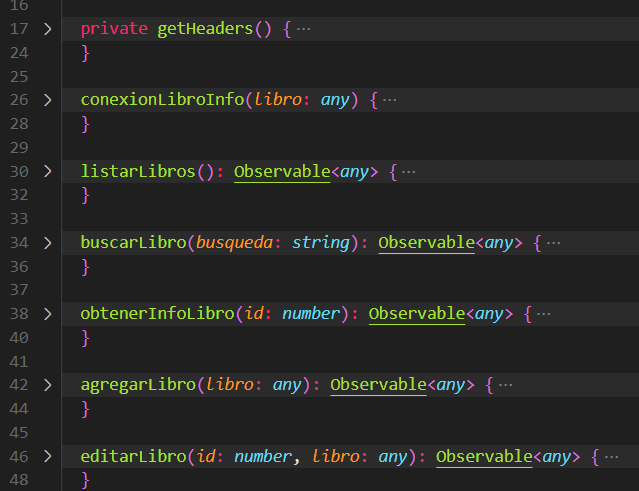
\includegraphics[width=0.7\linewidth]{Imagenes/LibroService.png}
    \caption{Servicio de libros}
    \label{Servicio de libros}
\end{figure}
\FloatBarrier

\newpage
\subsection{Patrones conjuntos}
\subsubsection{Patrón cliente-servidor~\cite{ModeloClienteServidor}}
Este último patrón es uno de los más importantes de este proyecto y se genera al existir de manera separada el \textit{backend} y el \textit{frontend}.
La forma en la que se muestra este patrón es de la siguiente manera:
\begin{itemize}
    \item Cliente: El cliente es el responsable de la interfaz de usuario, y en este proyecto recaería sobre la parte de Angular.
    \item Servidor: Son los responsables de devolver los recursos pedidos por los clientes, por lo que esta parte recaería sobre el \textit{backend} Flask.
\end{itemize}

El funcionamiento de este patrón se realiza mediante solicitudes HTTP por parte del cliente al servidor, los cuáles recibe el \textit{backend}, que procesa la información pedida utilizando parámetros recibidos del cliente (si existieran), y devuelve un resultado para que el cliente lo procese.


